\chapter{Mendix} \label{ch:mendix}
    Έχοντας πλέον μια καλή εικόνα για τον ορισμό του χαμηλού κώδικα και των Πλατφόρμων Ανάπτυξης Λογισμικού σε Low-Code, στο παρόν κεφάλαιο, θα επικεντρωθούμε σε μια από αυτές τις πλατφόρμες, το Mendix, η οποία αποτέλεσε το βασικό εργαλείο για την υλοποίηση της εφαρμογής που αναπτύχθηκε στο πλαίσιο της παρούσας διπλωματικής εργασίας. Θα...

%Σε αυτό το κεφάλαιο, θα παρουσιαστούν αναλυτικά οι βασικές λειτουργίες και τα χαρακτηριστικά της πλατφόρμας, καθώς και οι λόγοι που την καθιστούν κατάλληλη για την ανάπτυξη της συγκεκριμένης εφαρμογής. Επιπλέον, θα αναλυθούν τα εργαλεία που χρησιμοποιήθηκαν, οι τεχνολογίες που υποστηρίζει και τα πλεονεκτήματα που προσφέρει σε σχέση με άλλες παρόμοιες πλατφόρμες.

    \section{Τι είναι το Mendix;}
        Το Mendix αποτελεί μία από τις πιο διαδεδομένες πλατφόρμες ανάπτυξης λογισμικού που βασίζεται σε χαμηλό κώδικα. Ιδρύθηκε το 2005 στο Ρότερνταμ της Ολλανδίας με στόχο να παρέχει στους επιχειρηματίες και τους οργανισμούς τη δυνατότητα να αναπτύσσουν, να προσαρμόζουν και να διαχειρίζονται εφαρμογές αποδοτικά με χαμηλό κόστος. Το Mendix περιλαμβάνει όλα τα οφέλη και τα χαρακτηριστικά των LCDP που έχουν περιγραφτεί στην ενότητα \ref{sec:LCDP}, συμπεριλαμβάνοντας γραφικό περιβάλλον με WYSIWYG GUI σχεδιαστή, drag-and-drop εργαλεία και έτοιμες βιβλιοθήκες, τη χρήση domain models, το εύκολο deployment της εφαρμογής στο clout, version control μέσω Git, συνεργασία χρησιμοποιώντας Agile μεθοδολογία και άλλα.

        Το 2018, το Mendix εξαγοράστηκε από τη Siemens, τη μεγαλύτερη βιομηχανική κατασκευαστική εταιρεία στην Ευρώπη, γεγονός που επέφερε σημαντικές εξελίξεις στην πλατφόρμα. Η συγχώνευση αυτή επέτρεψε την ενσωμάτωση προηγμένων βιομηχανικών και IoT (Internet of Things) λύσεων, ενισχύοντας τη θέση του Mendix στην αγορά των λογισμικών σχεδιασμένων για επιχειρήσεις. Έτσι, το Mendix αποτελεί μία από τις πιο ισχυρές και ευέλικτες λύσεις στην αγορά του low-code προγραμματισμού, προσφέροντας αποτελεσματικότητα, ταχύτητα και καινοτομία στην ανάπτυξη λογισμικού, ενώ παράλληλα ενσωματώνει τις πιο σύγχρονες τεχνολογίες για να καλύψει τις ανάγκες επιχειρήσεων που επιθυμούν να παραμείνουν ανταγωνιστικές στην ψηφιακή εποχή. \cite{LowCodeMendix}

        Η Gartner, μία από τις μεγαλύτερες εταιρείες έρευνας και συμβουλευτικής στον κλάδο της τεχνολογίας, χαρακτηρίζει το Mendix ως ηγέτη στην αγορά των πλατφορμών ανάπτυξης λογισμικού για 8 συνεχόμενα χρόνια, (βλ. Σχήμα \ref{fig:GartnerQuadrant}). Η κατάταξη αυτή αποδεικνύει την ικανότητα του Mendix να παρέχει λύσεις υψηλής ποιότητας και αξίας στους πελάτες του, καθώς και την ικανότητά του να προσαρμόζεται στις ανάγκες της αγοράς και να προσφέρει συνεχώς καινοτόμες λύσεις. \cite{mendixGartnerQuadrant} Για αυτούς τους λόγους έχει προτιμηθεί για την υλοποίηση της εφαρμογής που θα παρουσιαστεί στο επόμενο κεφάλαιο.

            \begin{figure}[h!] \noindent \centering
                    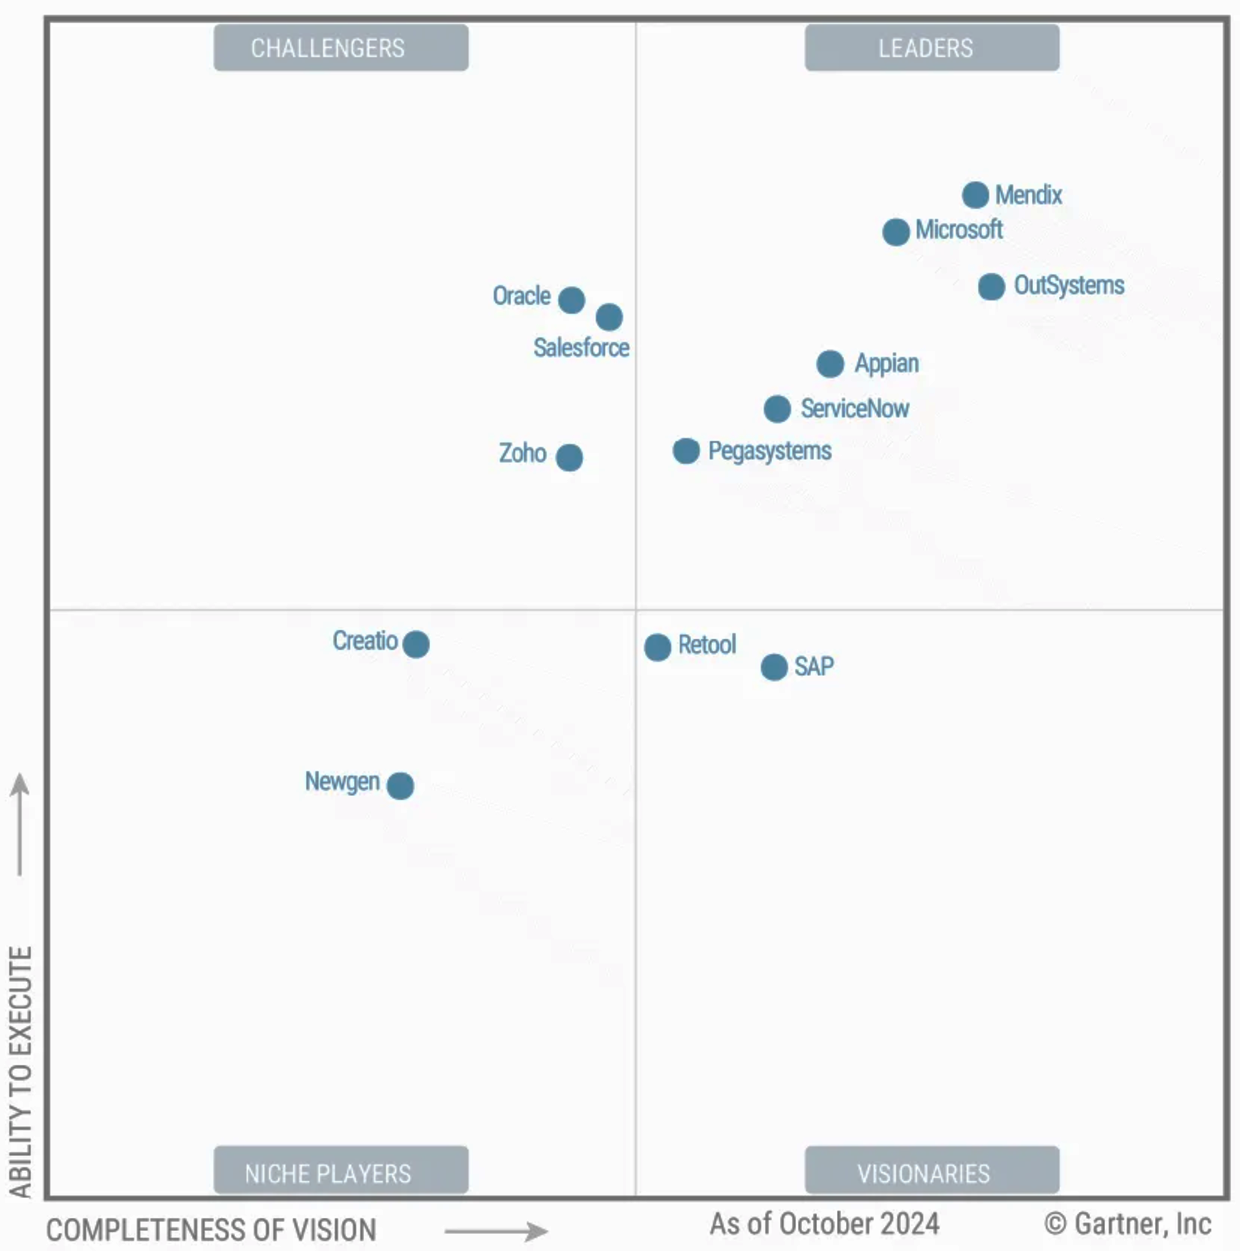
\includegraphics[width=0.5\textwidth]{GartnerQuadrant}
                    \caption{\centering Τεταρτημόριο της Gartner με πλατφόρμες ανάπτυξης λογισμικού \cite{mendixGartnerQuadrant}}
                    \label{fig:GartnerQuadrant}
            \end{figure}

    \section{<Χαρακτηριστικά Mendix>}

    \section{Το Mendix Studio}